\chapter{METODOLOGI}
\label{chap:desainimplementasi}

% Ubah bagian-bagian berikut dengan isi dari desain dan implementasi

Penelitian ini dilaksanakan sesuai desain sistem berikut beserta implementasinya.
Desain sistem merupakan konsep dari pembuatan dan perancangan infrastruktur dan kemudian
diwujudkan dalam bentuk blok-blok alur yang harus dikerjakan. Pada bagian implementasi merupakan
pelaksanaan teknis untuk setiap blok pada desain sistem.

% \section{Peralatan}
% \label{sec:peralatan}

% Peralatan yang digunakan selama pengerjaan tugas akhir ini yaitu Laptop untuk pengerjaan tugas akhir dari awal hingga penulisan buku dengan spesifikasi sebagai berikut

\section{Software}
\label{sec:software}

Sejumlah software digunakan sebagai pendukung pengerjaan Tugas Akhir ini.
Software yang berhubungan dengan Ethereum Blockchain diantaranya Remix,
Metamask, Ganache, dan Unreal Engine 5. Kemudian dari segi platform, yang digunakan adalah IPFS
dan Plugin-plugin yang ada di Unreal Engine 5 serta blueprintnya. Sementara dari Ethereum Blockchain,
bahasa pemrograman yang digunakan adalah Solidity.

% % Contoh pembuatan potongan kode
% \begin{lstlisting}[
%   language=C++,
%   caption={Program halo dunia.},
%   label={lst:halodunia}
% ]
% #include <iostream>

% int main() {
%     std::cout << "Halo Dunia!";
%     return 0;
% }
% \end{lstlisting}

\subsection{Remix IDE}
Remix adalah sebuah lingkungan pengembangan (IDE) yang populer dan terbuka untuk kontrak pintar (smart contract) Ethereum yang ditulis dalam bahasa Solidity. Remix menyediakan antarmuka yang intuitif dan lengkap untuk mengedit, menguji, dan menerapkan kontrak pintar secara langsung dari browser web tanpa perlu mengunduh atau menginstal perangkat lunak tambahan.

Remix menyediakan berbagai fitur yang memudahkan pengembangan kontrak pintar dalam bahasa Solidity. Beberapa fitur utama dari Remix meliputi:

\begin{enumerate}
  \item Editor Solidity: Remix menyediakan editor Solidity yang terintegrasi, yang memungkinkan pengembang untuk menulis, mengedit, dan memeriksa sintaksis dan kesalahan dalam kontrak pintar mereka. Editor ini juga menawarkan fitur seperti penyorotan sintaksis, penjajaran otomatis, dan saran kode (code completion) untuk mempercepat pengembangan.
  \item Penjelajah File: Remix memungkinkan pengembang untuk melihat struktur proyek mereka dengan menggunakan penjelajah file terintegrasi. Pengembang dapat dengan mudah menjelajahi dan mengatur file kontrak pintar, library, dan dependensi lainnya.
  \item Pemecah Masalah (Debugger): Remix dilengkapi dengan pemecah masalah yang kuat yang memungkinkan pengembang untuk menguji dan menganalisis langkah-demi-langkah eksekusi kontrak pintar. Dengan pemecah masalah, pengembang dapat memverifikasi logika dan perilaku kontrak pintar serta menemukan dan memperbaiki bug dengan lebih efisien.
  \item Simulasi dan Uji: Remix menyediakan fitur simulasi dan pengujian yang memungkinkan pengembang untuk menjalankan dan menguji kontrak pintar dalam lingkungan virtual sebelum diterapkan di jaringan Ethereum yang sebenarnya. Fitur ini membantu pengembang untuk mengidentifikasi dan memperbaiki masalah sebelum kontrak pintar diterapkan secara nyata.
  \item Integrasi Jaringan: Remix dapat terhubung ke berbagai jaringan Ethereum, termasuk jaringan pengembangan lokal seperti Ganache atau jaringan Ethereum utama. Ini memungkinkan pengembang untuk menguji dan menerapkan kontrak pintar pada berbagai lingkungan dengan mudah.
\end{enumerate}

Remix telah menjadi salah satu alat yang sangat populer dan diandalkan dalam komunitas pengembangan Ethereum. Antarmuka yang kuat dan berfitur lengkap, serta kemudahan penggunaan langsung dari browser, menjadikan Remix sebagai pilihan favorit bagi pengembang untuk mengembangkan, menguji, dan menerapkan kontrak pintar dalam bahasa Solidity.

\begin{figure}[H]
  \centering

  % Ubah dengan nama file gambar dan ukuran yang akan digunakan
  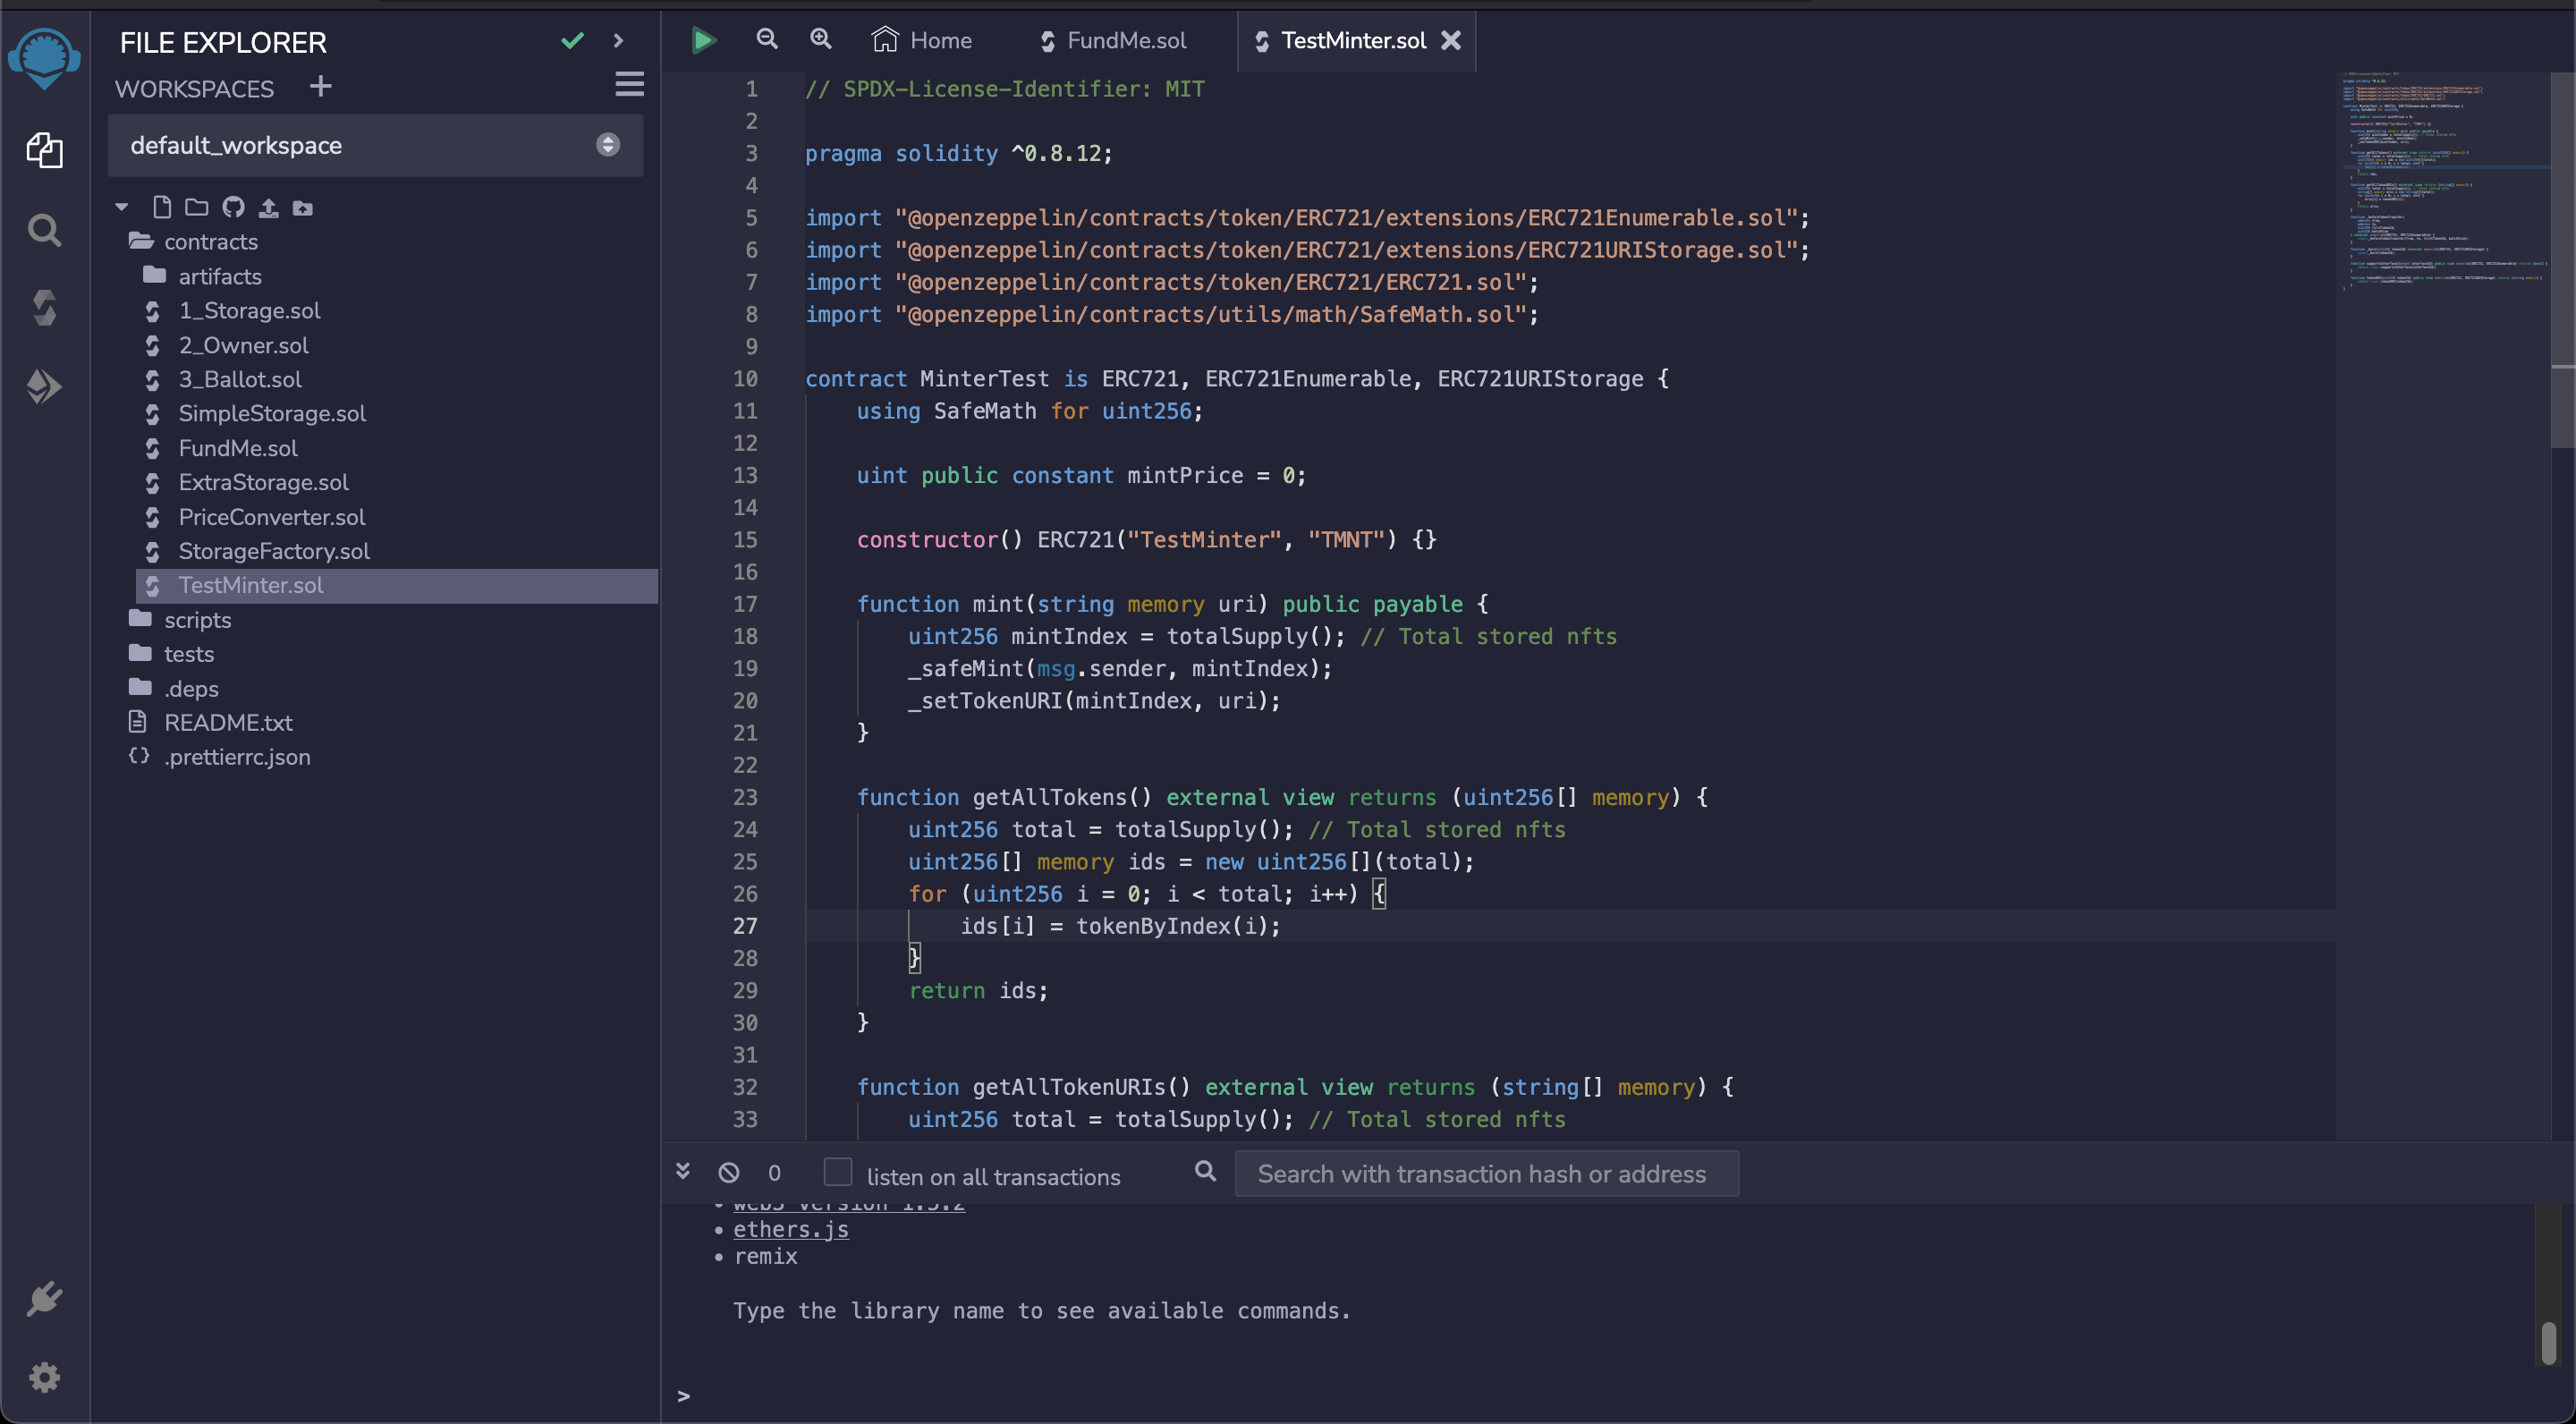
\includegraphics[scale=0.3]{gambar/remixide.png}

  % Ubah dengan keterangan gambar yang diinginkan
  \caption{Tampilan \emph{Remix IDE}.}
  \label{fig:remixide}
\end{figure}

\subsection{Ganache}
Ganache adalah sebuah perangkat lunak yang digunakan dalam pengembangan aplikasi berbasis blockchain, khususnya pada platform Ethereum. Ini adalah salah satu alat yang sangat populer di antara pengembang karena menyediakan lingkungan pengujian lokal yang mudah digunakan dan fleksibel.

Ganache awalnya dikenal dengan nama "TestRPC" sebelum berganti nama menjadi "Ganache". Perangkat lunak ini memungkinkan pengembang untuk melakukan pengembangan, pengujian, dan debugging aplikasi blockchain secara lokal tanpa perlu terhubung ke jaringan Ethereum yang sebenarnya. Dengan menggunakan Ganache, pengembang dapat membuat jaringan Ethereum pribadi mereka sendiri di mesin lokal mereka.

Berikut adalah beberapa fitur utama yang ditawarkan oleh Ganache:

\begin{enumerate}
  \item Jaringan Ethereum Lokal: Ganache menyediakan jaringan Ethereum lokal yang dapat dijalankan pada mesin pengembang. Jaringan ini berjalan di dalam lingkungan sandbox yang aman, yang memungkinkan pengembang untuk membuat dan menguji kontrak pintar, mentransaksikan token, dan menjalankan semua operasi yang terkait dengan Ethereum tanpa risiko kehilangan dana atau interaksi dengan jaringan utama.
  \item Blockchain Deterministik: Salah satu fitur kunci dari Ganache adalah kepastian (determinism) dari blockchain yang dihasilkan. Ini berarti bahwa setiap kali Ganache dijalankan dengan pengaturan yang sama, blockchain akan memiliki keadaan awal yang identik. Ini memungkinkan pengembang untuk menguji dan mengulangi skenario dengan hasil yang konsisten, yang sangat penting dalam pengujian dan debugging aplikasi blockchain.
  \item Mode Pembuatan Blok: Ganache menawarkan beberapa mode pembuatan blok yang dapat disesuaikan sesuai dengan kebutuhan pengembangan. Mode ini memungkinkan pengembang untuk mengendalikan bagaimana blok dibuat dan transaksi dikonfirmasi. Misalnya, pengembang dapat mengatur blok agar hanya dibuat setiap kali ada transaksi, atau mengatur kecepatan pembuatan blok agar sesuai dengan kecepatan transaksi yang diinginkan.
  \item Akun dan Kunci Pribadi: Ganache menyediakan sejumlah akun Ethereum yang siap digunakan dalam pengembangan. Setiap akun dilengkapi dengan kunci pribadi yang terkait, sehingga pengembang dapat menguji fungsi-fungsi yang melibatkan transaksi, seperti pengiriman Ether atau eksekusi kontrak pintar.
  \item Alat Pengembangan: Ganache dilengkapi dengan berbagai alat pengembangan yang membantu dalam memahami dan menganalisis aktivitas blockchain. Ini termasuk penjelajah blok (block explorer) yang memungkinkan pengembang untuk melihat detail transaksi dan status kontrak pintar, serta alat untuk melacak log dan debug kontrak pintar.
\end{enumerate}

Ganache dapat digunakan dalam berbagai skenario pengembangan, mulai dari pengujian kontrak pintar, pengembangan aplikasi terdesentralisasi, hingga pengujian keamanan. Dengan menggunakan Ganache, pengembang dapat dengan mudah membuat dan mengelola jaringan Ethereum lokal mereka sendiri, mempercepat siklus pengembangan, dan memastikan kualitas dan keandalan aplikasi blockchain yang dikembangkan.

\begin{figure}[H]
  \centering

  % Ubah dengan nama file gambar dan ukuran yang akan digunakan
  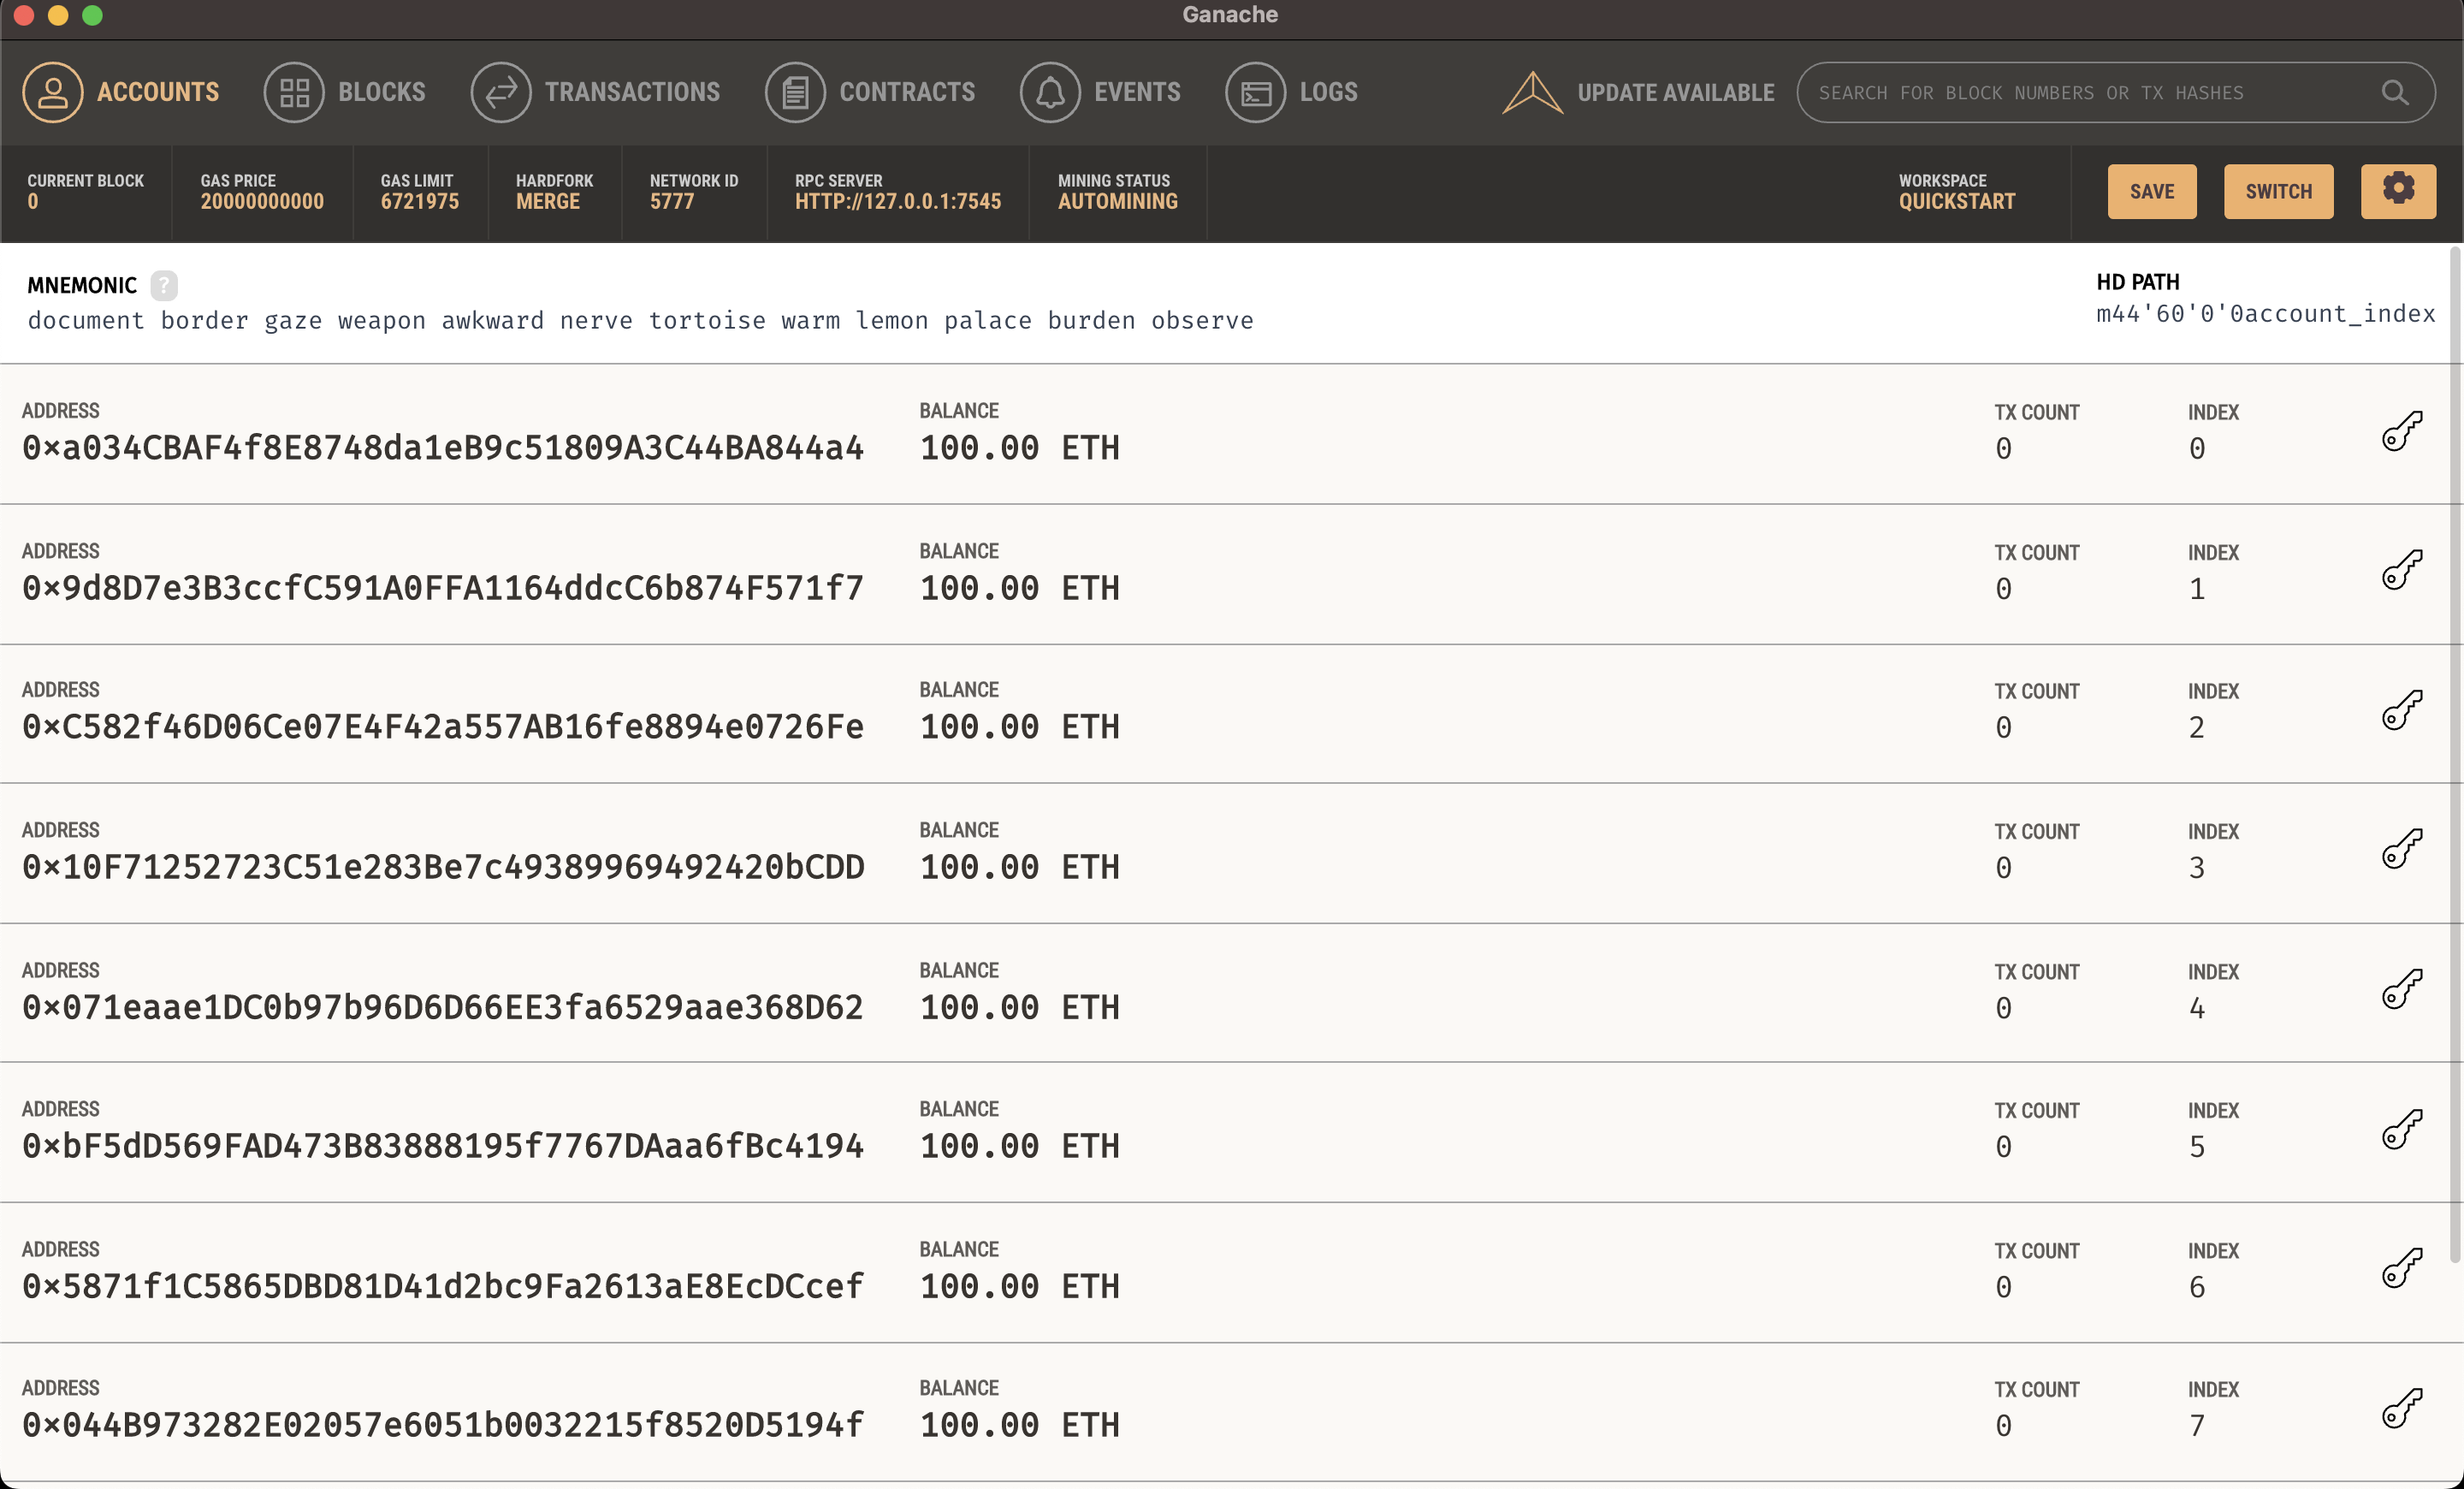
\includegraphics[scale=0.3]{gambar/ganache.png}

  % Ubah dengan keterangan gambar yang diinginkan
  \caption{Tampilan \emph{Ganache}.}
  \label{fig:ganache}
\end{figure}

\subsection{Unreal Engine 5}
Unreal Engine yang digunakan adalah versi 5.0.3. Unreal Engine digunakan untuk pengimplementasian \emph{Metaverse} yang mana dibuat sebuah lingkungan virtual sederhana seperti berikut.

\begin{figure}[H]
  \centering

  % Ubah dengan nama file gambar dan ukuran yang akan digunakan
  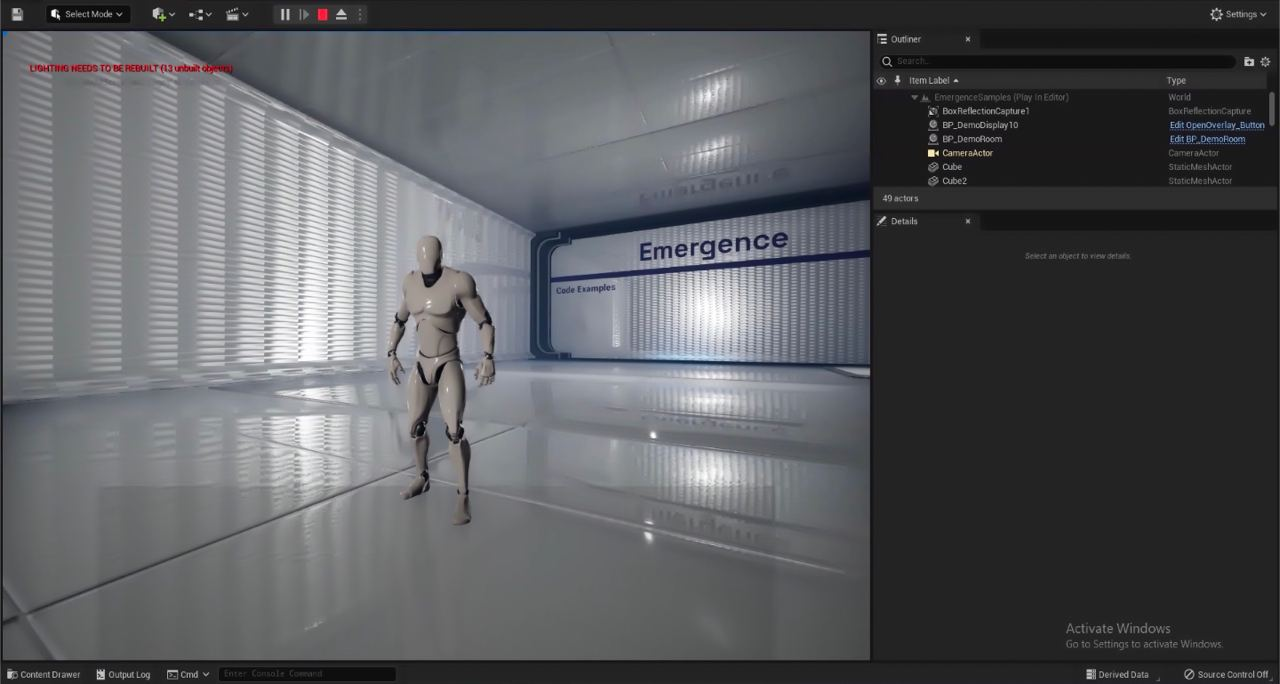
\includegraphics[scale=0.3]{gambar/ue5sample.jpg}

  % Ubah dengan keterangan gambar yang diinginkan
  \caption{Tampilan \emph{Unreal Engine 5}.}
  \label{fig:ue5sample}
\end{figure}

\section{Desain Sistem}

Tugas akhir ini dikerjakan dengan menggunakan beberapa service dan setiap service ini memiliki langkah-langkah tersendiri dalam pengerjaannya.
Untuk data \emph{raw} dari audionya disimpan di IPFS menggunakan Web3 Storage. Lalu untuk transmisi datanya menggunakan NFT yang akan di mint
dengan menggunakan protokol \emph{ERC-721}. Proses pembuatan NFT dilakukan dengan menggunakan smart contract yang ditulis dengan bahasa \emph{Solidity}

Penulisan \emph{Smart contract} dengan menggunakan \emph{solidity} dilakukan dengan menggunakan \emph{Remix IDE}.
\emph{Smart contract} yang ditulis diberikan beberapa \emph{method} tambahan yang akan membantu proses pengembangan dan integrasi ke \emph{Unreal Engine 5}

Setelah \emph{smart contract} ditulis, \emph{smart contract} dideploy. Kemudian dilakukan mint token dengan menggunakan tmapilan antarmuka dari Remix IDE.
Setelah sudah dilakukan deployment maka selanjutnya dilakukan pengintegrasian dengan Unreal Engine 5. NFT yang sudah di-mint dapat diperoleh dengan menggunakan
\emph{method smart contract} yang sudah ditulis sebelumnya. \emph{Metadata} yang tersimpan di NFT akan digunakan dan file audio yang terkandung didalamnya akan
di-play.

\begin{figure}[H]
  \centering

  % Ubah dengan nama file gambar dan ukuran yang akan digunakan
  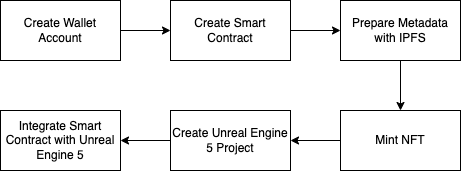
\includegraphics[scale=1]{gambar/desainsistem.png}

  % Ubah dengan keterangan gambar yang diinginkan
  \caption{Desain Sistem}
  \label{fig:desainsistem}
\end{figure}

\section{Create Wallet Account}

Proses pertama yang dilakukan adalah pembuatan akun wallet Ethereum dengan bantuan Metamask. Metamask merupakan sebuah plugin browser yang berfungsi sebagai
dompet penyimpanan Ethereum. Plugin ini dapat berinteraksi dengan Blockchain Ethereum yang didalamnya banyak terdapat aplikasi yang terdesentralisasi. Jaringan Ethereum dalam Metamask sangat beragam. Secara defaultnya, jaringan terdiri dari 2 jenis yakni Mainnet dan juga Testnet.

\begin{figure}[H]
  \centering

  % Ubah dengan nama file gambar dan ukuran yang akan digunakan
  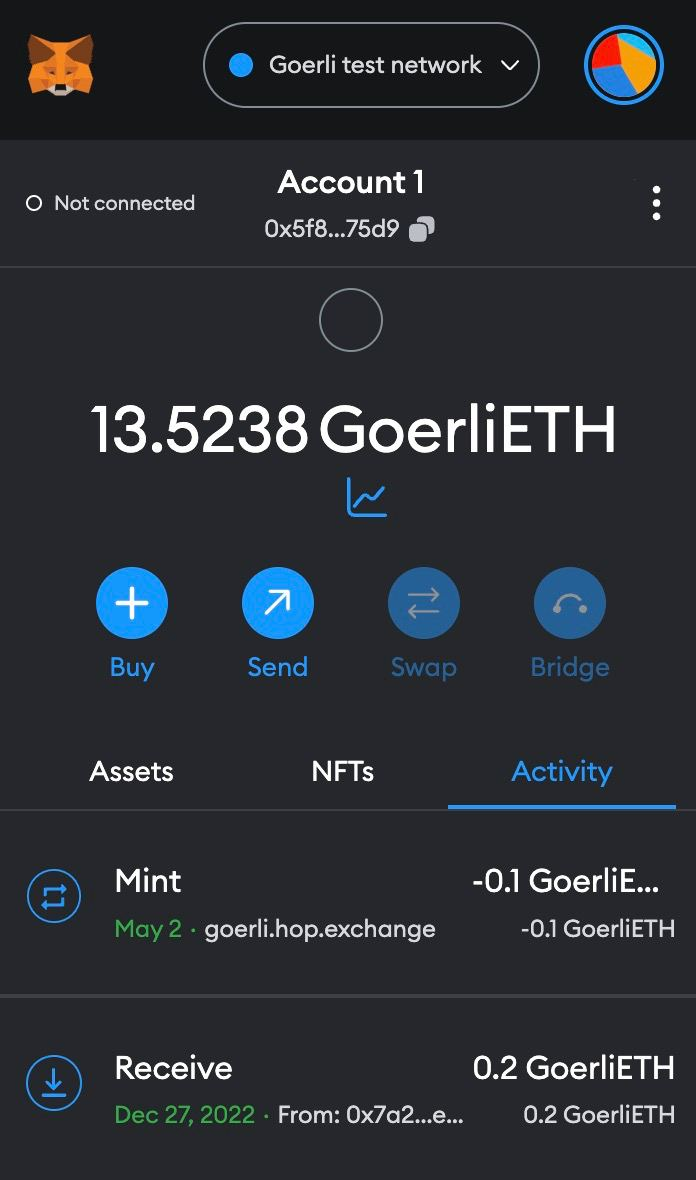
\includegraphics[scale=0.2]{gambar/tampilan-metamask.jpg}

  % Ubah dengan keterangan gambar yang diinginkan
  \caption{Tampilan Metamask}
  \label{fig:tampilanmetamask}
\end{figure}

Mainnet mengharuskan user untuk mengisi dompet Metamask dengan mata uang Ether asli, sehingga Metamask ini bisa digunakan untuk transaksi sehari-hari melewati jaringan Mainnet ini.
Sedangkan jaringan Testnet merupakan jaringan berbentuk perco- baan yang biasa digunakan untuk pengembangan aplikasi yang ingin diintegrasikan dengan Metamask. Pilihan Testnet ini juga tidak hanya satu, melainkan defaultnya terdapat
4 jaringan Testnet dalam Metamask, antara lain Ropsten, Goerli, Kovan, dan Rinkeby.

Masing-masing Testnet ini memiliki algoritma konsensus seperti Proof of Work dan Proof of Authority. Ropsten Testnet menggunakan algoritma Proof of Work dan Testnet lainnya menggunakan Proof of Authority. Untuk Proof of Stake dalam default plugin Metamask belum tersedia, namun Testnet dengan algoritma ini sudah tersedia seperti Kiln dan Kitsugi, dapat ditambahkan jaringannya pada Metamask.

Setelah membuat akun, akan diberikan Secret Recovery Phrase yang merupakan 12 kata unik dari Metamask sebagai cadangan untuk bisa masuk ke akun Metamask ketika password untuk login terlupakan. Secret Recovery Phrase ini dianjurkan untuk tidak disebarkan karena pengguna lain yang tidak memiliki akses ke password bisa mengakses akun Metamask orang lain hanya dengan Recovery Secret Phrase. Dalam plugin Metamask, pengguna dibebaskan membuat sejumlah akun lewat jaringan manapun. Untuk project ini, digunakan Testnet Ropsten yang menganut algoritma Proof of Work serta jaringan lokal Blockchain yang diperoleh dari Ganache sebagai mata uang untuk pengujian Smart Contract dan aplikasi.

Pada tahap ini, akun Testnet secara default akan memiliki 0 Ether, namun akun tersebut dapat memperoleh Ether dengan mencari faucet dari Testnet nya. Faucet ini nantinya yang akan mengirimkan sejumlah Ether sehingga akun Testnet bisa memperoleh Ether tanpa melakukan komputasi apapun. Maka dengan demikian, akun ini dinamakan Externally Owned Account, yang bisa dikendalikan langsung oleh pengguna tanpa perlu dikaitkan program. Nominal Testnet yang didapat hasil dari faucet bisa dikirimkan lang- sung ke akun lain di Testnet yang sama dengan fitur transfer between account, inilah fitur yang menjelaskan Externally Owned Account (EOA).

\begin{figure}[H]
  \centering

  % Ubah dengan nama file gambar dan ukuran yang akan digunakan
  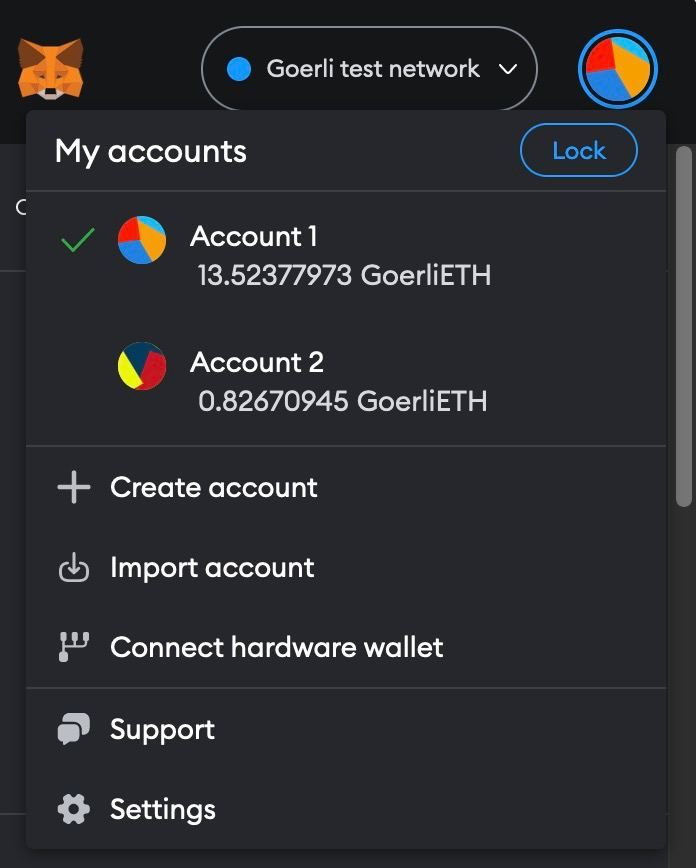
\includegraphics[scale=0.2]{gambar/akun-goerli.jpg}

  % Ubah dengan keterangan gambar yang diinginkan
  \caption{Tampilan Akun Goerli di Metamask}
  \label{fig:akungoerli}
\end{figure}

Akun wallet dari Metamask ini merupakan Ethereum Account yang dibuat dari kriptografis private dan public key. Dengan private key, membantu membuktikan bahwa transaksi benar-benar ditandatangani oleh pengirim dan mencegah pemalsuan. Public key dalam Metamask berarti sama dengan walllet address dari akun token Testnet yang digunakan (biasanya berawal dari 0x). Karena account Ethereum ini membutuhkan private
key untuk menandatangi transaksi agar bisa dikonfirmasi pada ledger, maka dari itu sistem ini menggunakan jenis yang sama pada sistem Multi Signature yaitu menggunakan 2 atau lebih private key untuk menandatangi transaksi dari akun yang berbeda. Komparasi dengan sistem wallet di Indonesia saat ini menunjukan perbedaan dimana di Indonesia, sistemnya saat ini menggunakan 2 factor authentication dengna OTP dan juga PIN untuk melakukan transaksi sehingga media nya berbeda. Tetapi pada sistem layanan uang digital di Indonesia masih bersifat sentralisasi, sedangkan pada Multi Signature karena memanfaatkan teknologi Blockchain Ethereum, bersifat desentralisasi. Pada implementasinya, Multi Signature dapat menggunakan prinsip 2FA dengan cara menggunakan device yang berbeda. Satu orang dapat mengimplementasikan sistem ini jika memiliki lebih dari satu device untuk melakukan koneksi ke wallet yang sudah memiliki sistem Multi Signature

\section{Create \emph{Smart Contract}}

Pembuatan Smart Contract merupakan salah satu kelebihan dari Ethereum, dimana fitur didalam wallet Ether semua diprogram dalam Smart Contract sesuai dengan kebutuhan.
Token yang akan digunakan adalah token dengan spesifikasi ERC-721 atau disebut juga dengan NFT (Non Fungible Token)
Pertama ditentukan spesifikasi token ERC-721 yang ingin dibuat. Ini meliputi pengaturan seperti nama token, simbol, dan jumlah total token yang akan dikeluarkan.
Dapat juga dipertimbangkan apakah perlu menyertakan metadata tambahan seperti deskripsi, gambar, atau atribut khusus.
Kontrak pintar (smart contract) harus dibuat menggunakan bahasa pemrograman Solidity dengan library standar ERC-721 diimpor dan kontrak didefinisikan sebagai kontrak yang mengimplementasikan interface ERC-721.
Fungsi-fungsi utama seperti transfer token, melihat informasi token, dan lainnya perlu diatur. Logika bisnis yang diinginkan perlu diimplementasikan pada token ERC-721. Uji dan rilis harus dilakukan untuk memastikan kontrak berfungsi sebagaimana yang diharapkan.
Kontrak dapat diuji secara lokal menggunakan alat pengujian seperti Ganache atau Remix sebelum dirilis ke jaringan Ethereum.

Dalam smart contract yang dibuat, diberikan method-method tambahan seperti \texttt{tokenURI}, \texttt{getAllTokens}, dan \texttt{getAllTokenURIs}.

% Contoh input potongan kode dari file
\lstinputlisting[
  language=Solidity,
  caption={Smart Contract untuk Mint NFT.},
  label={lst:bilanganprima}
]{program/TestMinter.sol}

Listing diatas adalah kontrak smart contract Solidity yang menggunakan beberapa kontrak dari library OpenZeppelin untuk mengimplementasikan ERC-721, ERC-721Enumerable, dan ERC-721URIStorage. Berikut adalah pembahasan secara lebih rinci setiap bagian dari kode tersebut:

\subsection{Kontrak Import dan Inheritance}
Kontrak menggunakan @openzeppelin/contracts library untuk mengimpor kontrak ERC721, ERC721Enumerable, dan ERC721URIStorage. Kontrak MinterTest adalah turunan dari ketiga kontrak tersebut.
\subsection{Konstruktor}
Konstruktor digunakan untuk menginisialisasi kontrak dengan memberikan nama dan simbol untuk token ERC-721 yang dibuat.
Dalam kode ini, konstruktor didefinisikan menggunakan fungsi constructor() dengan menggunakan konstruktor kontrak ERC721.

\subsection{Fungsi Mint}
Fungsi mint digunakan untuk membuat token baru dan meng-assign kepemilikannya kepada pengirim transaksi.
Fungsi ini menerima parameter uri yang merupakan URI unik untuk token yang akan dibuat.
Setelah token dibuat, fungsi \_safeMint digunakan untuk mengalokasikan token kepada pengirim transaksi.
Fungsi \_setTokenURI digunakan untuk mengatur URI token.

\subsection{Fungsi getAllTokens}
Fungsi getAllTokens digunakan untuk mengembalikan array dengan daftar semua token yang ada dalam kontrak.
Fungsi ini menggunakan fungsi totalSupply untuk mendapatkan total jumlah token yang ada.
Kemudian, dalam loop, fungsi tokenByIndex digunakan untuk mendapatkan ID token pada indeks tertentu.

\subsection{Fungsi getAllTokenURIs}
Fungsi getAllTokenURIs digunakan untuk mengembalikan array dengan daftar URI semua token dalam kontrak.
Fungsi ini juga menggunakan fungsi totalSupply untuk mendapatkan total jumlah token yang ada.
Dalam loop, fungsi tokenURI digunakan untuk mendapatkan URI token pada indeks tertentu.

\subsection{Fungsi \_beforeTokenTransfer dan \_burn}
Fungsi \_beforeTokenTransfer dan \_burn merupakan fungsi internal yang di-override dari kontrak ERC721 dan ERC721URIStorage.
Fungsi \_beforeTokenTransfer dijalankan sebelum token transfer terjadi.
Fungsi \_burn dijalankan saat token di-burn (dihapus) dari kontrak.

\subsection{Fungsi supportsInterface dan tokenURI}
Fungsi supportsInterface dan tokenURI adalah fungsi yang di-override dari kontrak ERC721 dan ERC721URIStorage.
Fungsi supportsInterface memeriksa apakah kontrak mendukung interface tertentu.
Fungsi tokenURI mengembalikan URI token berdasarkan ID token yang diberikan.

Setelah dilakukan penulisan kode solidity maka dapat dilakukan deployment. Deployment dilakukan dengan environment \emph{Injected Provider - Metamask}


\begin{figure}[H]
  \centering

  % Ubah dengan nama file gambar dan ukuran yang akan digunakan
  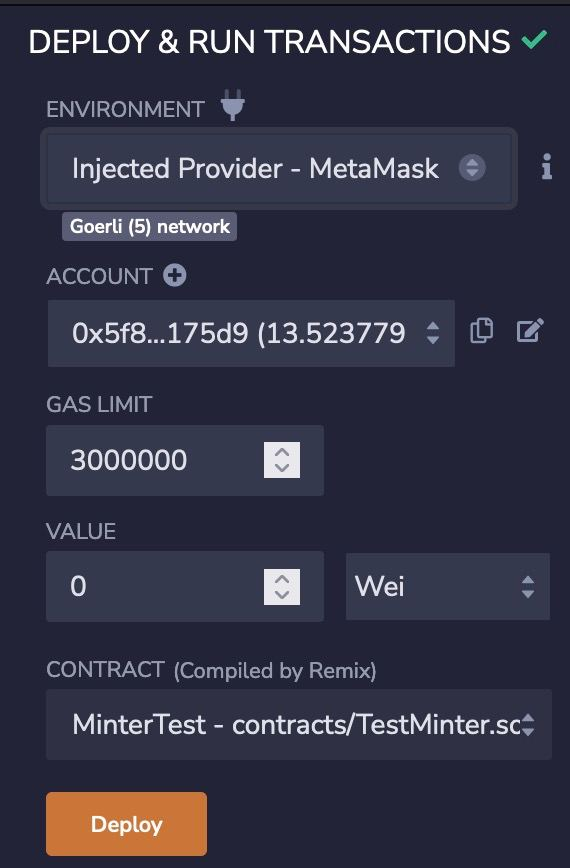
\includegraphics[scale=0.4]{gambar/deployment-interface.jpg}

  % Ubah dengan keterangan gambar yang diinginkan
  \caption{Antarmuka Deployment di Remix IDE}
  \label{fig:deploymentinterface}
\end{figure}

\section{Prepare Metadata with IPFS}

Untuk melakukan persiapan metadata, maka perlu ditentukan dulu format JSON yang akan digunakan. Format JSON yang digunakan adalah format dari
OpenSea yang adalah seperti berikut.


\begin{figure}[H]
  \centering

  % Ubah dengan nama file gambar dan ukuran yang akan digunakan
  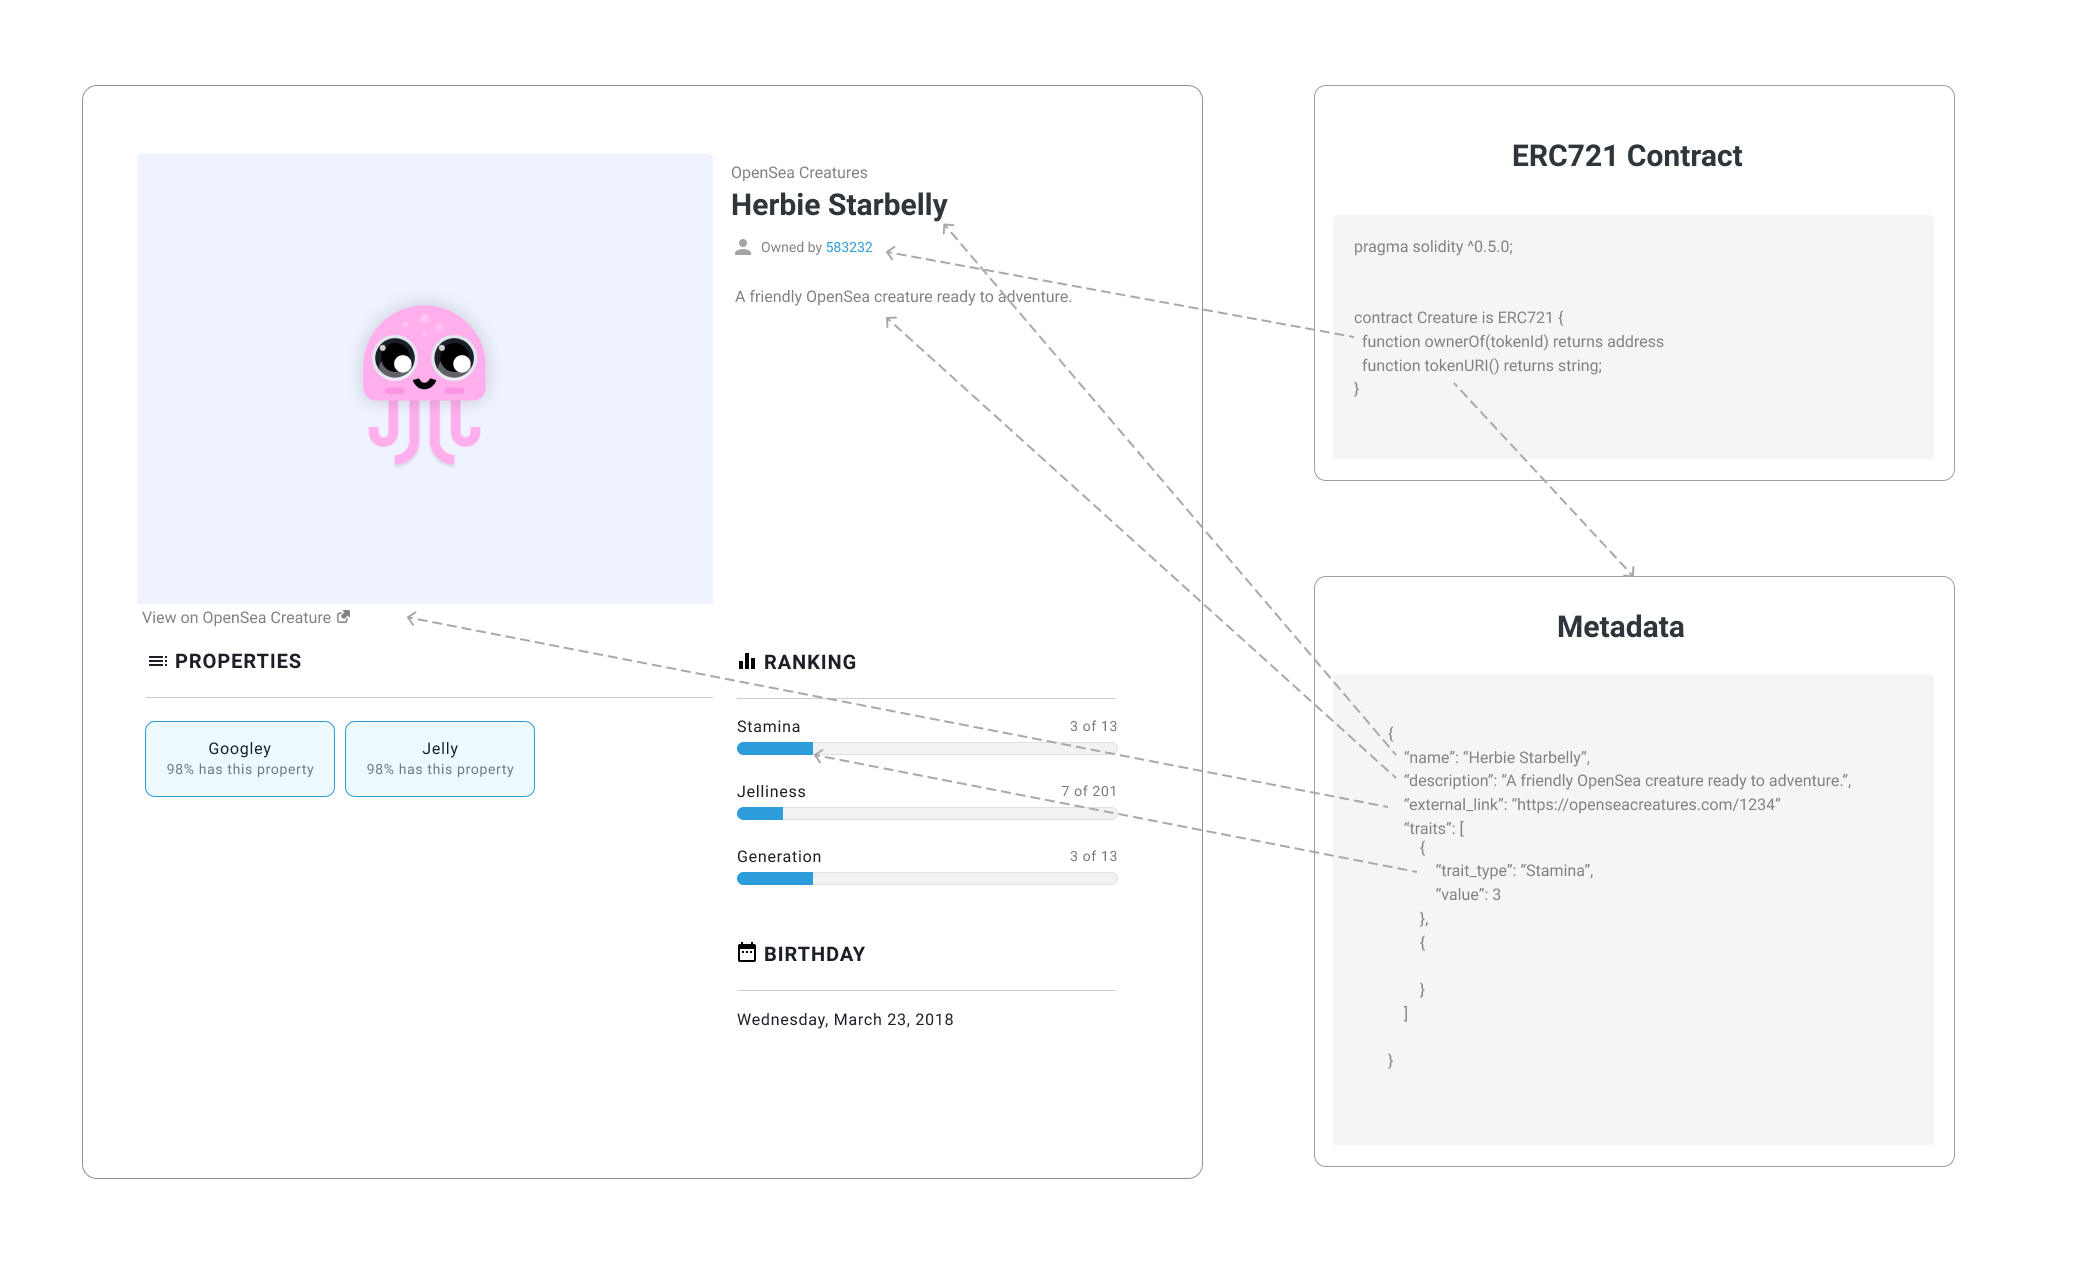
\includegraphics[scale=0.23]{gambar/nft-standards-opensea.png}

  % Ubah dengan keterangan gambar yang diinginkan
  \caption{Standar NFT OpenSea}
  \label{fig:openseanft}
\end{figure}

Dari struktur metadata tersebut, dibuatlah beberapa modifikasi dan tambahan field seperti audio\_url untuk menampung URL dari audio yang digunakan.
\lstinputlisting[
  language=json,
  caption={Format JSON untuk metadata NFT.},
  label={lst:nftformat}
]{program/nft-1.json}

\subsection{Web3 Storage}
Service IPFS yang digunakan adalah Web3 Storage. Semua asset-asset yang akan digunakan diunggah di Web3 Storage.

web3.storage adalah kumpulan API dan layanan yang memudahkan pengembang dan pengguna lain untuk berinteraksi dengan data tanpa terikat pada lokasi fisik penyimpanan data tersebut. Layanan ini secara asli menggunakan protokol data dan identitas terdesentralisasi seperti IPFS, Filecoin, dan UCAN yang memungkinkan arsitektur dan alur kerja aplikasi yang berfokus pada verifikasi data dan pengguna.

Di inti platform ini terdapat layanan penyimpanan terhosting yang dapat digunakan untuk mengunggah dan menyimpan data agar tetap tersedia secara berkelanjutan. Platform ini juga menyediakan layanan tambahan seperti w3link dan w3name yang memudahkan pembuatan pengalaman web yang mulus dan menyenangkan dengan memanfaatkan protokol web3.

\begin{figure}[H]
  \centering

  % Ubah dengan nama file gambar dan ukuran yang akan digunakan
  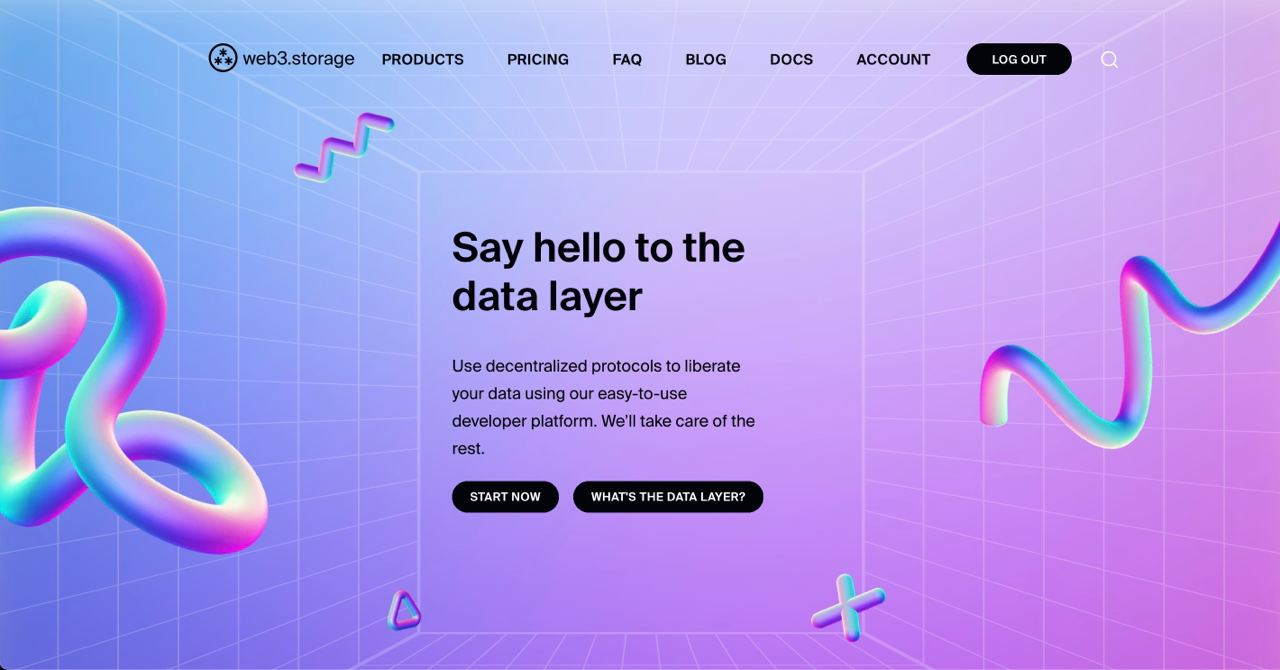
\includegraphics[scale=0.3]{gambar/web3storage.jpg}

  % Ubah dengan keterangan gambar yang diinginkan
  \caption{Tampilan web3.storage}
  \label{fig:web3storage}
\end{figure}

Dengan menggunakan web3.storage akan diupload file-file yang akan digunakan untuk data dari sistem.
Data-data atau assets ini menggunakan audio yang berlisensi CC0.

\begin{figure}[H]
  \centering

  % Ubah dengan nama file gambar dan ukuran yang akan digunakan
  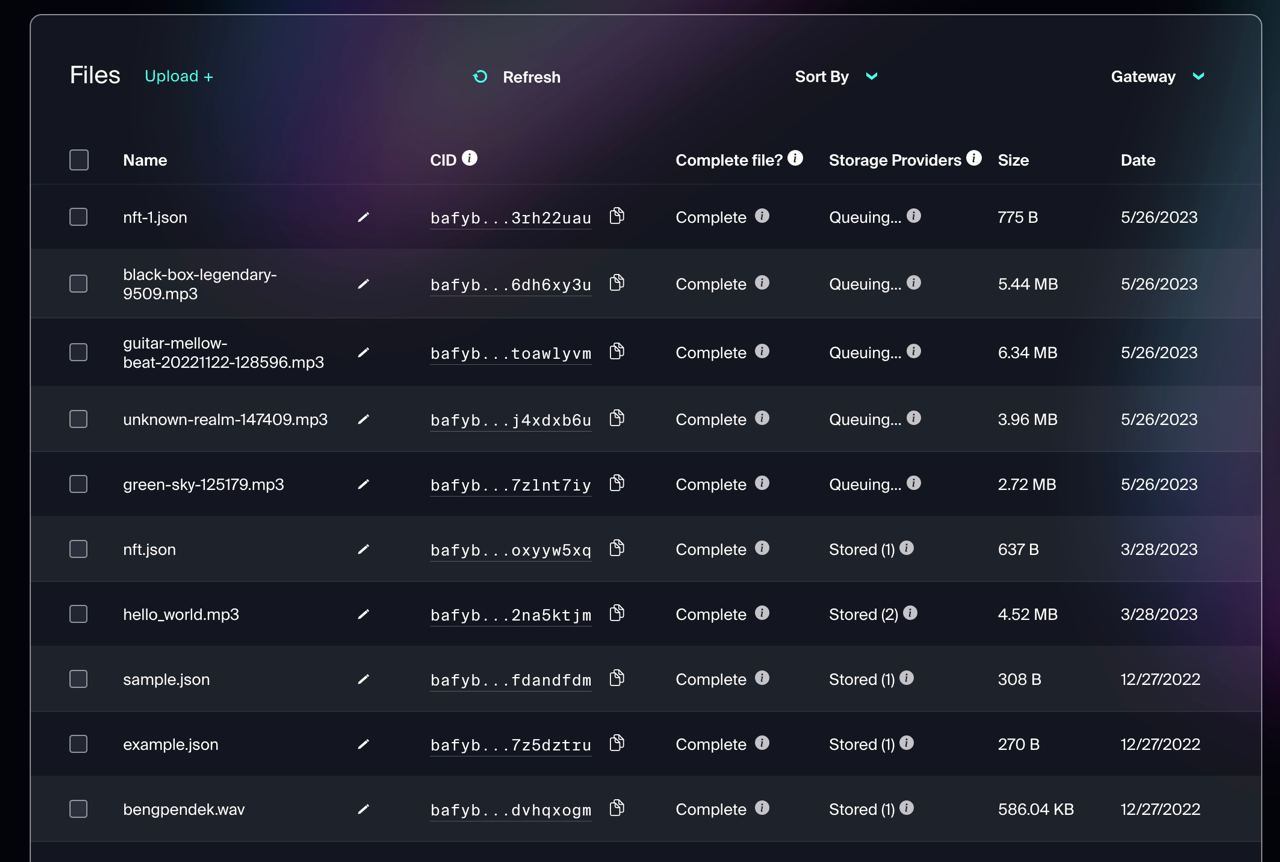
\includegraphics[scale=0.3]{gambar/web3storageacc.jpg}

  % Ubah dengan keterangan gambar yang diinginkan
  \caption{Tampilan di menu file web3.storage}
  \label{fig:web3storageacc}
\end{figure}

Url dari audio yang sudah diupload akan diletakkan kedalam Metadata json, kemudian json tersebut akan diupload juga
ke web3.storage.

\section{Mint NFT}

Di tahap ini dilakukan proses mint NFT dengan menggunakan \emph{smart contract} yang sudah dideploy sebelumnya.
Remix IDE sudah menyediakan antarmuka untuk memanggil method-method yang ada di smart contract yang sudah terdeploy.

\begin{figure}[H]
  \centering

  % Ubah dengan nama file gambar dan ukuran yang akan digunakan
  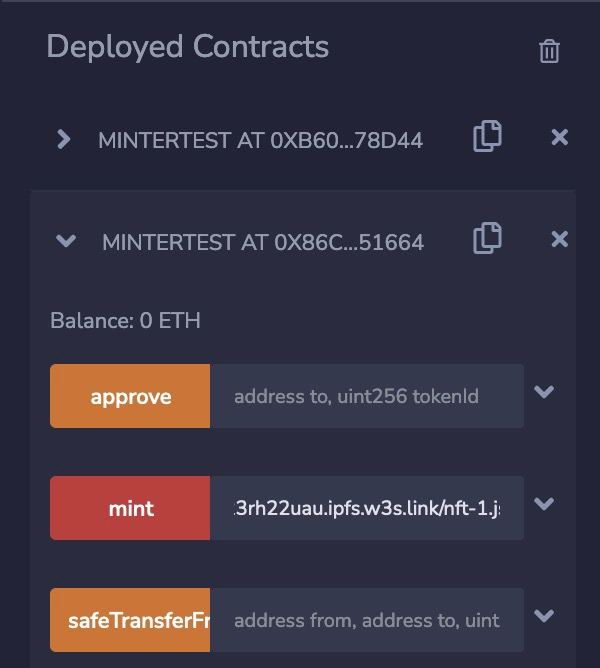
\includegraphics[scale=0.3]{gambar/mint-nft.jpg}

  % Ubah dengan keterangan gambar yang diinginkan
  \caption{Tampilan Remix IDE untuk deployed contracts}
  \label{fig:mintnft}
\end{figure}

Dapat juga dicek melalui etherscan. Domain etherscan yang digunakan adalah milik goerli karena wallet yang digunakan juga menggunakan goerli.
Etherscan Goerli adalah sebuah platform yang memberikan berbagai macam layanan dan utilitas yang berguna dalam pengembangan smart contract di jaringan Goerli, yang merupakan salah satu jaringan pengujian pada Ethereum. Platform ini menyediakan berbagai fitur yang memungkinkan pengembang untuk menjelajahi, memantau, dan menganalisis smart contract dan transaksi yang terjadi di jaringan Goerli.

Salah satu kegunaan utama dari Etherscan Goerli adalah untuk menjelajahi dan menganalisis smart contract. Pengembang dapat menggunakan platform ini untuk melihat detail dari suatu smart contract, termasuk kode sumbernya, fungsi-fungsi yang ada, dan variabel-variabel yang digunakan. Informasi ini sangat penting dalam memahami dan memeriksa kecerdasan kontrak sebelum diterapkan di jaringan Ethereum utama. Selain itu, Etherscan Goerli juga menyediakan alat untuk memeriksa riwayat transaksi, sehingga pengembang dapat melacak aliran nilai dan interaksi yang terjadi pada suatu smart contract.

Selain menjelajahi dan menganalisis smart contract, Etherscan Goerli juga menyediakan utilitas untuk memantau dan melacak kinerja dan keadaan jaringan Goerli. Pengembang dapat memeriksa informasi tentang blok terbaru, hash blok, kecepatan transaksi, dan pemegang akun. Ini membantu pengembang dalam mengamati performa jaringan dan memastikan bahwa transaksi yang mereka kirimkan berjalan dengan baik di jaringan pengujian.

Selain itu, Etherscan Goerli juga memberikan fitur untuk memverifikasi smart contract. Pengembang dapat mengirimkan kode sumber smart contract mereka ke platform ini untuk diverifikasi. Dengan melakukan verifikasi, pengembang dapat memastikan bahwa smart contract yang mereka kembangkan sesuai dengan apa yang diharapkan, dan memastikan bahwa tidak ada perubahan yang tidak diinginkan atau malware yang dimasukkan ke dalam kontrak.

Selain fitur-fitur utama di atas, Etherscan Goerli juga menyediakan berbagai informasi terkait dengan jaringan Goerli, seperti harga gas, grafik transaksi, dan pemantauan kontrak yang populer. Semua informasi ini membantu pengembang dalam memperoleh pemahaman yang lebih baik tentang jaringan Goerli dan membantu mereka dalam mengembangkan dan menguji smart contract dengan lebih efektif.

Dalam pengembangan smart contract, Etherscan Goerli memberikan alat yang sangat berharga untuk menjelajahi, memantau, menganalisis, dan memverifikasi smart contract di jaringan Goerli. Dengan menggunakan platform ini, pengembang dapat memperoleh wawasan yang mendalam tentang keadaan jaringan, memeriksa dan memverifikasi kecerdasan kontrak, serta memastikan performa yang baik dalam pengujian smart contract sebelum diterapkan di jaringan Ethereum utama.

\section{Create Unreal Engine 5 Project}

Proyek Unreal Engine 5 dibuat dengan mengikuti serangkaian langkah yang penting dan harus diikuti dengan cermat. Pertama, Unreal Engine 5 diinstal dari situs resmi Epic Games dan memastikan persyaratan sistem yang diperlukan terpenuhi oleh komputer. Setelah diinstal, Unreal Engine Launcher dibuka dan proyek baru dibuat dengan memilih jenis proyek yang sesuai dengan tujuan. Setelah masuk ke Unreal Editor, pengaturan proyek dikonfigurasi seperti resolusi layar, sistem fisika, kontrol input, dan lainnya sesuai kebutuhan.

Selanjutnya, dunia (World) dibuat di mana permainan atau pengalaman berlangsung. Alat bawaan Unreal Engine 5 seperti Landscape Editor digunakan untuk membuat lingkungan yang realistis dengan menambahkan peta, objek, karakter, dan lainnya. Selanjutnya, objek dan karakter dibuat atau diimpor ke dalam proyek. Aset dapat dibuat sendiri atau model 3D yang sudah ada diimpor dalam berbagai format seperti FBX atau OBJ. Setelah itu, animasi, tekstur, suara, dan perilaku yang diinginkan ditambahkan.

Selanjutnya, bahasa pemrograman visual bernama Blueprint digunakan untuk membuat logika permainan. Dengan Blueprint, alur permainan, skrip perilaku objek, pengaturan kamera, penanganan interaksi pemain, dan lainnya dapat dibuat. Jika memiliki pengetahuan dalam pemrograman C++, bahasa ini juga dapat digunakan dalam pengembangan proyek. Efek visual dan suara juga dapat diterapkan menggunakan fitur dan alat bawaan Unreal Engine 5, seperti pencahayaan, partikel, efek cuaca, dan suara latar.

Setelah proyek selesai dibuat, pengujian dan iterasi dilakukan. Proyek dijalankan di Unreal Editor atau mode standalone untuk melihat bagaimana proyek berjalan, bug diidentifikasi dan diperbaiki, serta pengujian dilakukan untuk memastikan kualitas dan kinerja yang baik. Terakhir, setelah proyek selesai dan telah diuji dengan baik, proyek dapat didistribusikan kepada pengguna akhir. Unreal Engine 5 menyediakan berbagai opsi distribusi, termasuk platform PC, konsol, dan virtual reality (VR), sesuai dengan kebutuhan proyek.

Proyek Unreal Engine yang dibuat sederhana saja, namun tetap dapat berinteraksi dengan menggunakan blueprints.

Kemudian perlu juga menambahkan beberapa plugin yang akan digunakan nantinya seperti Runtime Audio Importer, IPFS, dan Emergence.

\subsection{Runtime Audio Importer}
Runtime Audio Importer adalah sebuah fitur yang memungkinkan pengguna untuk mengimpor audio dalam berbagai format secara langsung saat berjalan. Fitur ini menawarkan kecepatan transkoding yang cepat dan mendukung format audio utama seperti MP3, WAV, FLAC, OGG Vorbis, dan BINK. Selain itu, fitur ini juga mendukung format RAW seperti int8, uint8, int16, uint16, int32, uint32, dan float32.

Runtime Audio Importer memiliki perilaku yang sama dengan gelombang suara biasa, termasuk SoundCue dan MetaSounds (mulai dari versi 5.2). Fitur ini juga secara otomatis mendeteksi format audio yang digunakan dan mendukung fungsionalitas streaming audio. Selain itu, pengguna juga dapat menangkap audio dari perangkat input seperti mikrofon, mengekspor gelombang suara ke file terpisah, dan menggunakan aset suara yang telah diimpor sebelumnya.

Yang menarik, Runtime Audio Importer tidak membutuhkan pustaka statis atau dependensi eksternal tertentu. Fitur ini mendukung semua perangkat yang tersedia seperti Android, iOS, Windows, Mac, Linux, dan sebagainya.

\subsection{Emergence}
Emergence adalah protokol Web3 yang ditujukan untuk pengembang game, yang terintegrasi dengan mesin permainan seperti Unreal Engine dan Unity melalui SDK berbasis Web3. Emergence memberdayakan pengembang game dengan otentikasi dompet, smart contract, sistem avatar, dan layanan inventaris NFT. Alat yang mudah digunakan dan kreatif memungkinkan pemain untuk masuk dengan mudah menggunakan dompet kripto mereka dan bermain dengan persona pilihan mereka secara transparan. Sementara itu, Emergence memberikan alat kepada pengembang game untuk memanfaatkan item NFT pengguna dan menyematkannya ke dalam permainan mereka secara mulus.

Protokol Emergence menyediakan alat yang diperlukan agar para pencipta dapat membangun dunia-dunia yang interoperabel, di mana pengguna dapat membuat persona berbasis rantai blok mereka sendiri dan memuat avatar, inventaris, dan data ke dalam dunia metaverse pilihan mereka.

Dengan menyediakan alat seperti Layanan Inventaris, para pencipta dapat melihat potensi NFT dari segi utilitas. Bukan hanya dalam desain aslinya, tetapi juga dengan mempertimbangkan penggunaan NFT sebagai GameObjects aktual dalam dunia virtual mereka. Pengembang dapat menggunakan Layanan Inventaris Emergence untuk menyimpan metadata dinamis ke dalam NFT pengguna mereka. Hal ini membuka peluang besar untuk memikirkan tentang gaming berbasis Web3 yang baru dan apa yang dapat dicapai oleh NFT, serta bagaimana NFT tersebut berkembang melalui pengalaman metaverse. NFT lebih dari sekadar PFP (profil foto). Mereka dapat dianggap sebagai objek permainan yang persisten dan interoperabel, membawa inovasi baru dalam penceritaan, interaksi, pengalaman, dan sebagainya.

SDK Emergence menyediakan akses kode tingkat rendah dan tingkat tinggi untuk berinteraksi dengan jaringan EVM (Ethereum Virtual Machine) dan dompet. Mulai dari mengotentikasi pengguna dengan tanda tangan digital yang memungkinkan bentuk otentikasi universal baru, hingga membaca dan menulis ke smart contract. Dengan menyediakan alat seperti Sistem Avatar dan Layanan Inventaris, Emergence memberikan serangkaian fungsi agar pencipta metaverse apa pun dapat dengan mudah memanfaatkan kekuatan Web3.

\section{Integrate Smart Contract with Unreal Engine 5}

Proses integrasi smart contract dengan Unreal Engine 5 ini membutuhkan pengetahuan tentang blueprints. Proses ini dimulai dengan menyiapkan kembali proyek Unreal Engine 5
Dengan menggunakan plugin Emergence kita dapat menentukan contract dan juga menghubungkan blueprints dengan contracts yang sudah dideploy.

Plugin ini memiliki asset-asset yang akan membantu seperti asset contract dan deployed contract.

\begin{figure}[H]
  \centering

  % Ubah dengan nama file gambar dan ukuran yang akan digunakan
  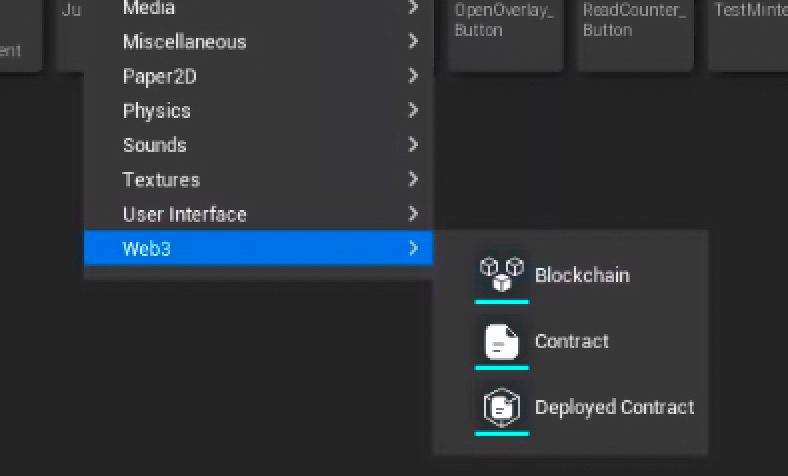
\includegraphics[scale=0.3]{gambar/web3emergence.jpg}

  % Ubah dengan keterangan gambar yang diinginkan
  \caption{Tampilan Asset yang disediakan Emergence}
  \label{fig:web3emergence}
\end{figure}

Emergence contract asset digunakan oleh berbagai metode dan objek sebagai deskriptor antarmuka pemrograman suatu kontrak. Sebagian besar datanya berasal dari ABI (Application Binary Interface) kontrak tersebut.

Aset Kontrak Emergence merujuk pada komponen yang digunakan oleh berbagai metode dan objek dalam ekosistem Emergence untuk menjelaskan antarmuka pemrograman suatu kontrak. Aset ini berfungsi sebagai deskriptor yang memberikan informasi penting tentang struktur kontrak, fungsi, dan data yang terkait. Sebagian besar data yang terkait dengan aset ini berasal dari ABI kontrak, yang mendefinisikan bagaimana kontrak dapat diinteraksikan dan diakses oleh entitas eksternal.

Aset Kontrak Emergence memainkan peran penting dalam memfasilitasi integrasi dan interaksi yang lancar antara berbagai komponen dalam ekosistem Emergence. Dengan memanfaatkan ABI kontrak, pengembang dapat berkomunikasi dan berinteraksi dengan kontrak pintar secara efektif, memungkinkan mereka untuk memanggil fungsi spesifik, mengambil data, dan melakukan operasi lain yang didefinisikan dalam antarmuka kontrak.

Data yang disimpan dalam Aset Kontrak Emergence mencakup informasi seperti tanda tangan fungsi kontrak, parameter masukan dan keluaran, definisi acara, dan metadata lain yang diperlukan untuk berinteraksi dengan kontrak. Data ini memungkinkan komponen lain dalam ekosistem Emergence, seperti kontrak pintar, aplikasi, atau antarmuka pengguna, untuk memahami dan memanfaatkan fungsionalitas yang ditawarkan oleh kontrak.

Secara keseluruhan, Aset Kontrak Emergence berfungsi sebagai deskriptor yang menggambarkan antarmuka pemrograman suatu kontrak dalam ekosistem Emergence. Mereka memungkinkan integrasi, komunikasi, dan interaksi yang lancar dengan kontrak pintar dengan menyediakan informasi penting yang berasal dari ABI kontrak. Dengan memanfaatkan aset ini, pengembang dapat efektif menggunakan fungsionalitas yang ditawarkan oleh kontrak dan membangun aplikasi terdesentralisasi dan layanan inovatif dalam ekosistem Emergence.

\begin{figure}[H]
  \centering

  % Ubah dengan nama file gambar dan ukuran yang akan digunakan
  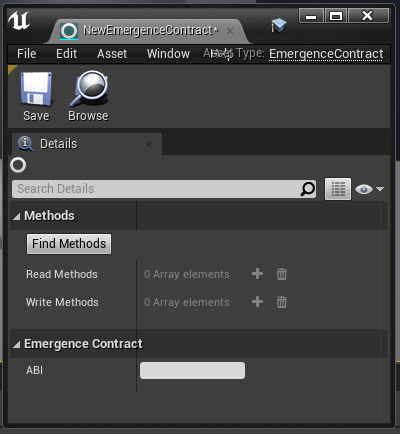
\includegraphics[scale=0.6]{gambar/emergencecontract.png}

  % Ubah dengan keterangan gambar yang diinginkan
  \caption{Tampilan Asset Kontrak Emergence}
  \label{fig:emergencecontract}
\end{figure}

Aset Kontrak Emergence yang Dideploy digunakan oleh berbagai metode dan objek sebagai referensi ke kontrak tertentu yang telah dideploy di dalam blockchain. Aset ini terdiri dari aset Blockchain, aset Kontrak, dan alamat kontrak.

Aset Kontrak Emergence yang Dideploy adalah komponen yang digunakan dalam ekosistem Emergence untuk mengidentifikasi dan berinteraksi dengan kontrak pintar yang telah dideploy di dalam blockchain. Aset ini mencakup informasi yang penting untuk mengarahkan aplikasi atau komponen lain ke kontrak yang tepat untuk berinteraksi dengannya.

Komponen utama dari Aset Kontrak Emergence yang Dideploy adalah aset Blockchain yang merujuk pada blockchain tempat kontrak dideploy, aset Kontrak yang menggambarkan kontrak pintar secara keseluruhan, dan alamat kontrak yang merupakan alamat unik yang menunjukkan lokasi kontrak di dalam blockchain.

Dengan menggunakan Aset Kontrak Emergence yang Dideploy, pengembang dapat dengan mudah mengakses kontrak pintar yang telah dideploy di dalam blockchain. Mereka dapat memanggil fungsi kontrak, membaca dan menulis data, serta berinteraksi dengan kontrak untuk menjalankan logika bisnis yang diinginkan.

Secara keseluruhan, Aset Kontrak Emergence yang Dideploy berfungsi sebagai referensi yang mengarahkan aplikasi atau komponen lain ke kontrak pintar yang telah dideploy di dalam blockchain. Dengan menggunakan informasi yang terkandung dalam aset ini, pengembang dapat secara efisien berinteraksi dengan kontrak pintar dan memanfaatkan fungsionalitas yang ditawarkan oleh kontrak tersebut dalam ekosistem Emergence.

\begin{figure}[H]
  \centering

  % Ubah dengan nama file gambar dan ukuran yang akan digunakan
  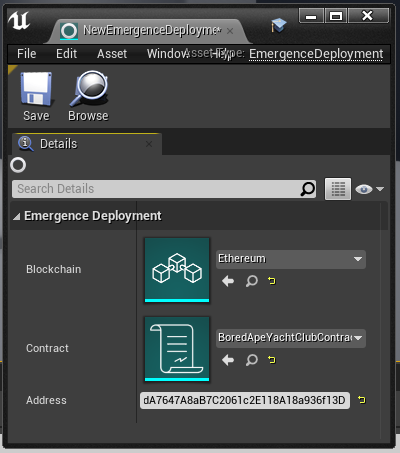
\includegraphics[scale=0.6]{gambar/emergencedeployedcontract.png}

  % Ubah dengan keterangan gambar yang diinginkan
  \caption{Tampilan Deployed Contracts dari Emergence}
  \label{fig:emergencedeployedcontract}
\end{figure}

Dari asset-asset tersebut akan diread oleh blueprint component dari emergence.

\subsection{Read Method}

\begin{figure}[H]
  \centering

  % Ubah dengan nama file gambar dan ukuran yang akan digunakan
  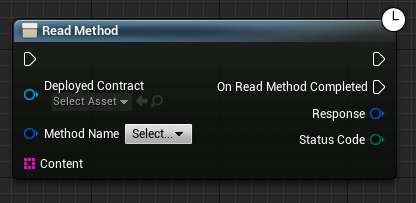
\includegraphics[scale=0.6]{gambar/readmethod.png}

  % Ubah dengan keterangan gambar yang diinginkan
  \caption{Tampilan Blueprint Read Method}
  \label{fig:readmethod}
\end{figure}

Read method ini memiliki kegunaan untuk memanggil read method pada smart contract yang diberikan. Disini diberikan
input berupa smart contract yang dideploy, nama method, dan content yaitu parameter yang akan diberikan pada method smart contract.

Kemudian dari method tersebut akan mendecode NFT yang didapat dan mendapatkan format metadata. Di metadata tersebut akan terdapat field \texttt{audio\_url}.
Field ini mengandung link url ke asset audio. Audio ini kemudian dapat diproses dan diplay dengan blueprints pada Unreal Engine 5.
